\documentclass[a4paper,10pt]{article}
\usepackage[applemac]{inputenc} %\usepackage[utf8]{inputenc}
\usepackage[pdftex]{graphicx}

\title{Arduino Laser Actuator}
\author{InThe - Aclaro}
\date{2012-09-01}

\pdfinfo{%
  /Title    (Arduino L�ser Actuator)
  /Author   (Josep)
  /Creator  ()
  /Producer ()
  /Subject  ()
  /Keywords ()
}

\begin{document}
\maketitle

\section{Objectiu}

\section{}

\subsection{Arduino}
Arduino �s una plataforma de codi obert (\emph{opensource}) de desnvolupament de prototips electr�nics. L

\begin{figure}[htbp] %  figure placement: here, top, bottom, or page
   \centering
	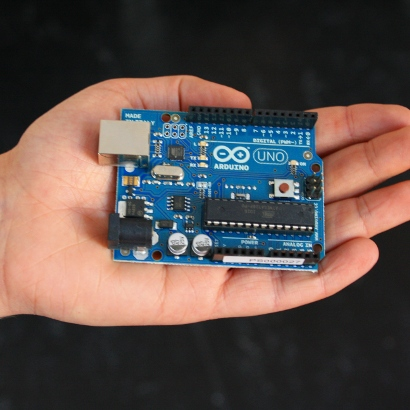
\includegraphics[scale=0.5]{images/arduino_uno_test.jpg} 
   \caption{Placa Arduino Uno}
   \label{fig:example}
\end{figure}

\end{document}
